\documentclass{standalone}
\usepackage{tikz}
\usepackage{xcolor}
\usetikzlibrary{patterns, positioning}
\usetikzlibrary{shapes.misc}
\usepackage[outline]{contour}
\contourlength{1.5pt} 


\begin{document}
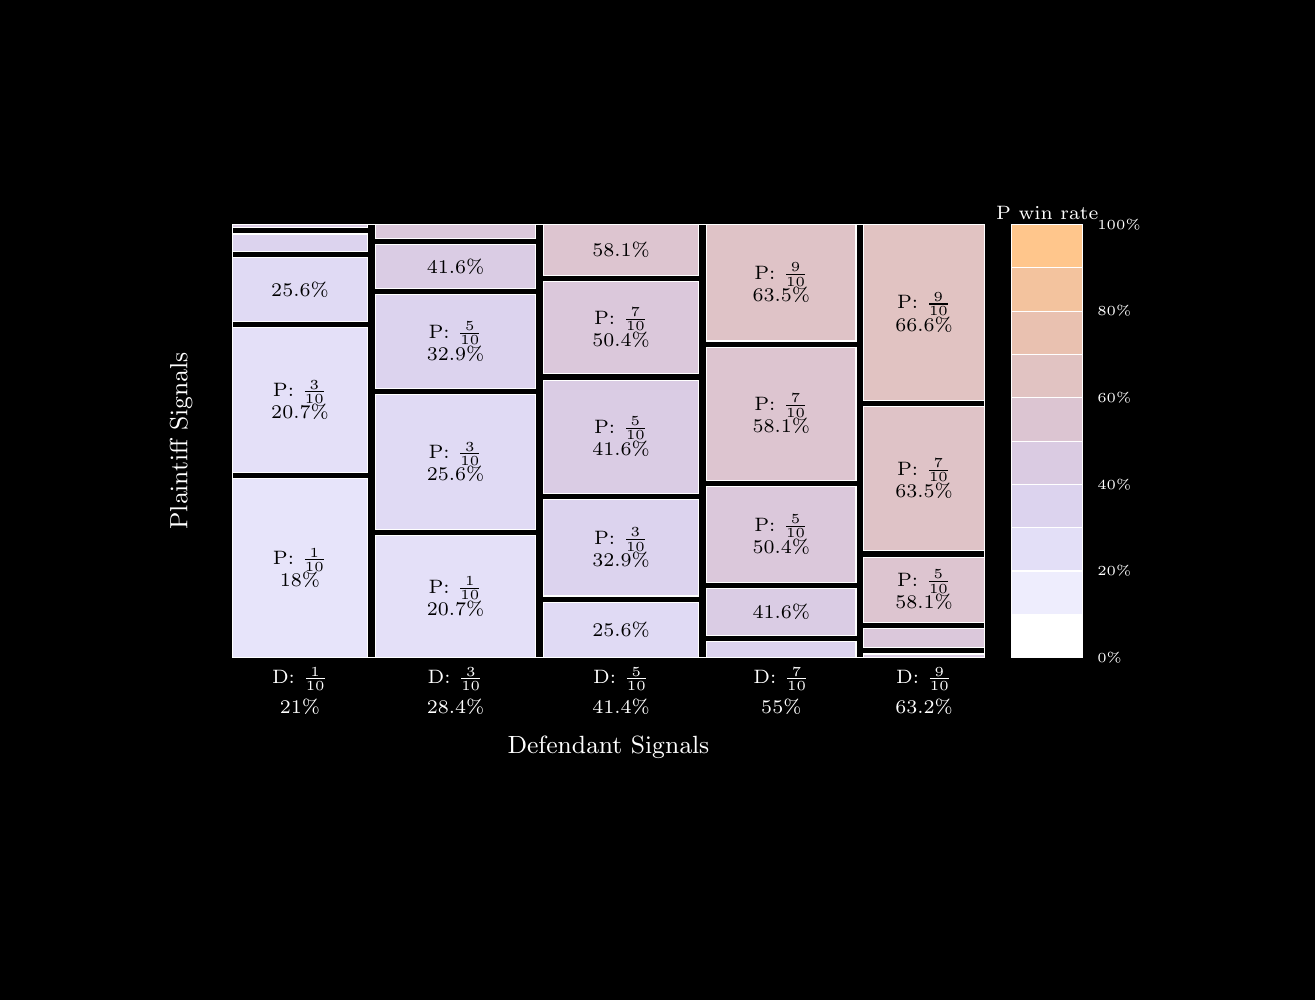
\begin{tikzpicture}
\newcommand{\DFractionOffset}{0.4}
\newcommand{\AxisLabelYAdjust}{-0.235}
\pagecolor{black}
\draw[fill=black, draw=none] (-2,-2) rectangle (14,10);
\draw[draw=white] (0.6,2) rectangle (10.15,7.5);
\draw[fill=blue!82!orange!18!white!65!white, draw=white] (0.6,2) rectangle (2.317,4.2757);
\draw (1.4584821675843567, 3.1378726591505774) node[font=\scriptsize, text=black, align=center] {P: $\frac{1}{10}$\\ 18\%};
\draw[fill=blue!79!orange!21!white!65!white, draw=white] (0.6,4.3557) rectangle (2.317,6.1904);
\draw (1.4584821675843567, 5.273063175011099) node[font=\scriptsize, text=black, align=center] {P: $\frac{3}{10}$\\ 20.7\%};
\draw[fill=blue!74!orange!26!white!64!white, draw=white] (0.6,6.2704) rectangle (2.317,7.0773);
\draw (1.4584821675843567, 6.673846239760312) node[font=\scriptsize, text=black, align=center] {25.6\%};
\draw[fill=blue!67!orange!33!white!62!white, draw=white] (0.6,7.1573) rectangle (2.317,7.3789);
\draw[fill=blue!58!orange!42!white!60!white, draw=white] (0.6,7.4589) rectangle (2.317,7.5);
\draw (1.4584821675843567, 1.6) node[anchor=north, font=\scriptsize, text=white] {21\%};
\draw (1.4584821675843567, {1.6 + \DFractionOffset}) node[anchor=north, font=\scriptsize, text=white] {D: $\frac{1}{10}$};
\draw[fill=blue!79!orange!21!white!65!white, draw=white] (2.417,2) rectangle (4.4512,3.5485);
\draw (3.434059886221792, 2.7742645429692683) node[font=\scriptsize, text=black, align=center] {P: $\frac{1}{10}$\\ 20.7\%};
\draw[fill=blue!74!orange!26!white!64!white, draw=white] (2.417,3.6285) rectangle (4.4512,5.341);
\draw (3.434059886221792, 4.48477485510924) node[font=\scriptsize, text=black, align=center] {P: $\frac{3}{10}$\\ 25.6\%};
\draw[fill=blue!67!orange!33!white!62!white, draw=white] (2.417,5.421) rectangle (4.4512,6.6059);
\draw (3.434059886221792, 6.0134789436540395) node[font=\scriptsize, text=black, align=center] {P: $\frac{5}{10}$\\ 32.9\%};
\draw[fill=blue!58!orange!42!white!60!white, draw=white] (2.417,6.6859) rectangle (4.4512,7.241);
\draw (3.434059886221792, 6.963454678462538) node[font=\scriptsize, text=black, align=center] {41.6\%};
\draw[fill=blue!50!orange!50!white!57!white, draw=white] (2.417,7.321) rectangle (4.4512,7.5);
\draw (3.434059886221792, 1.6) node[anchor=north, font=\scriptsize, text=white] {28.4\%};
\draw (3.434059886221792, {1.6 + \DFractionOffset}) node[anchor=north, font=\scriptsize, text=white] {D: $\frac{3}{10}$};
\draw[fill=blue!74!orange!26!white!64!white, draw=white] (4.5512,2) rectangle (6.5233,2.7025);
\draw (5.5372209724791, 2.3512623390398573) node[font=\scriptsize, text=black, align=center] {25.6\%};
\draw[fill=blue!67!orange!33!white!62!white, draw=white] (4.5512,2.7825) rectangle (6.5233,4.0047);
\draw (5.5372209724791, 3.393626779620027) node[font=\scriptsize, text=black, align=center] {P: $\frac{3}{10}$\\ 32.9\%};
\draw[fill=blue!58!orange!42!white!60!white, draw=white] (4.5512,4.0847) rectangle (6.5233,5.5245);
\draw (5.5372209724791, 4.8046325977048205) node[font=\scriptsize, text=black, align=center] {P: $\frac{5}{10}$\\ 41.6\%};
\draw[fill=blue!50!orange!50!white!57!white, draw=white] (4.5512,5.6045) rectangle (6.5233,6.7743);
\draw (5.5372209724791, 6.1894252574454836) node[font=\scriptsize, text=black, align=center] {P: $\frac{7}{10}$\\ 50.4\%};
\draw[fill=blue!42!orange!58!white!55!white, draw=white] (4.5512,6.8543) rectangle (6.5233,7.5);
\draw (5.5372209724791, 7.177157100320832) node[font=\scriptsize, text=black, align=center] {58.1\%};
\draw (5.5372209724791, 1.6) node[anchor=north, font=\scriptsize, text=white] {41.4\%};
\draw (5.5372209724791, {1.6 + \DFractionOffset}) node[anchor=north, font=\scriptsize, text=white] {D: $\frac{5}{10}$};
\draw[fill=blue!67!orange!33!white!62!white, draw=white] (6.6233,2) rectangle (8.5198,2.2006);
\draw[fill=blue!58!orange!42!white!60!white, draw=white] (6.6233,2.2806) rectangle (8.5198,2.8759);
\draw (7.571557751364754, 2.5782792791600837) node[font=\scriptsize, text=black, align=center] {41.6\%};
\draw[fill=blue!50!orange!50!white!57!white, draw=white] (6.6233,2.9559) rectangle (8.5198,4.1723);
\draw (7.571557751364754, 3.5641388242107217) node[font=\scriptsize, text=black, align=center] {P: $\frac{5}{10}$\\ 50.4\%};
\draw[fill=blue!42!orange!58!white!55!white, draw=white] (6.6233,4.2523) rectangle (8.5198,5.9405);
\draw (7.571557751364754, 5.096423015731661) node[font=\scriptsize, text=black, align=center] {P: $\frac{7}{10}$\\ 58.1\%};
\draw[fill=blue!36!orange!64!white!54!white, draw=white] (6.6233,6.0205) rectangle (8.5198,7.5);
\draw (7.571557751364754, 6.760253467377975) node[font=\scriptsize, text=black, align=center] {P: $\frac{9}{10}$\\ 63.5\%};
\draw (7.571557751364754, 1.6) node[anchor=north, font=\scriptsize, text=white] {55\%};
\draw (7.571557751364754, {1.6 + \DFractionOffset}) node[anchor=north, font=\scriptsize, text=white] {D: $\frac{7}{10}$};
\draw[fill=blue!58!orange!42!white!60!white, draw=white] (8.6198,2) rectangle (10.15,2.0461);
\draw[fill=blue!50!orange!50!white!57!white, draw=white] (8.6198,2.1261) rectangle (10.15,2.3641);
\draw[fill=blue!42!orange!58!white!55!white, draw=white] (8.6198,2.4441) rectangle (10.15,3.2763);
\draw (9.384914497523088, 2.8601884054231403) node[font=\scriptsize, text=black, align=center] {P: $\frac{5}{10}$\\ 58.1\%};
\draw[fill=blue!36!orange!64!white!54!white, draw=white] (8.6198,3.3563) rectangle (10.15,5.19);
\draw (9.384914497523088, 4.273143503717281) node[font=\scriptsize, text=black, align=center] {P: $\frac{7}{10}$\\ 63.5\%};
\draw[fill=blue!33!orange!67!white!53!white, draw=white] (8.6198,5.27) rectangle (10.15,7.5);
\draw (9.384914497523088, 6.385004412147925) node[font=\scriptsize, text=black, align=center] {P: $\frac{9}{10}$\\ 66.6\%};
\draw (9.384914497523088, 1.6) node[anchor=north, font=\scriptsize, text=white] {63.2\%};
\draw (9.384914497523088, {1.6 + \DFractionOffset}) node[anchor=north, font=\scriptsize, text=white] {D: $\frac{9}{10}$};
\node[font=\small, text=white] at (5.375, {1.1 + \AxisLabelYAdjust}) {Defendant Signals};
\node[font=\small, text=white, rotate=90] at (-0.050000000000000044, 4.75) {Plaintiff Signals};
\draw[draw=white] (10.5,2) rectangle (11.4,7.5);
\draw (10.95, 7.65) node[font=\scriptsize, text=white] {P win rate};
\draw[fill=blue!100!orange!0!white!70!white, draw=white] (10.5,2) rectangle (11.4,2.55);
\draw[fill=blue!89!orange!11!white!67!white, draw=white] (10.5,2.55) rectangle (11.4,3.1);
\draw[fill=blue!78!orange!22!white!64!white, draw=white] (10.5,3.1) rectangle (11.4,3.65);
\draw[fill=blue!67!orange!33!white!62!white, draw=white] (10.5,3.65) rectangle (11.4,4.2);
\draw[fill=blue!56!orange!44!white!59!white, draw=white] (10.5,4.2) rectangle (11.4,4.75);
\draw[fill=blue!44!orange!56!white!56!white, draw=white] (10.5,4.75) rectangle (11.4,5.3);
\draw[fill=blue!33!orange!67!white!53!white, draw=white] (10.5,5.3) rectangle (11.4,5.85);
\draw[fill=blue!22!orange!78!white!51!white, draw=white] (10.5,5.85) rectangle (11.4,6.4);
\draw[fill=blue!11!orange!89!white!48!white, draw=white] (10.5,6.4) rectangle (11.4,6.95);
\draw[fill=blue!0!orange!100!white!45!white, draw=white] (10.5,6.95) rectangle (11.4,7.5);
\draw (11.46, 2) node[anchor=west, font=\tiny, text=white] {0\%};
\draw (11.46, 3.1) node[anchor=west, font=\tiny, text=white] {20\%};
\draw (11.46, 4.2) node[anchor=west, font=\tiny, text=white] {40\%};
\draw (11.46, 5.3) node[anchor=west, font=\tiny, text=white] {60\%};
\draw (11.46, 6.4) node[anchor=west, font=\tiny, text=white] {80\%};
\draw (11.46, 7.5) node[anchor=west, font=\tiny, text=white] {100\%};


\end{tikzpicture}
\end{document}